\section{The Data Model Design}

The purpose of class diagrams in systems design is that they are a visual way to represent the internal data structure model of an object oriented program. They provide a forward plan for the complex hierarchies of a program and allow you to build up a compositional view and begin thinking about access availability\cite{fowleruml}. They do not provide implementation details, but when a design is modular and composable enough the overall method structure will provide a high detail and can imply underlying implementations in a clear and concise way.

\begin{figure}[H]
    \centering
    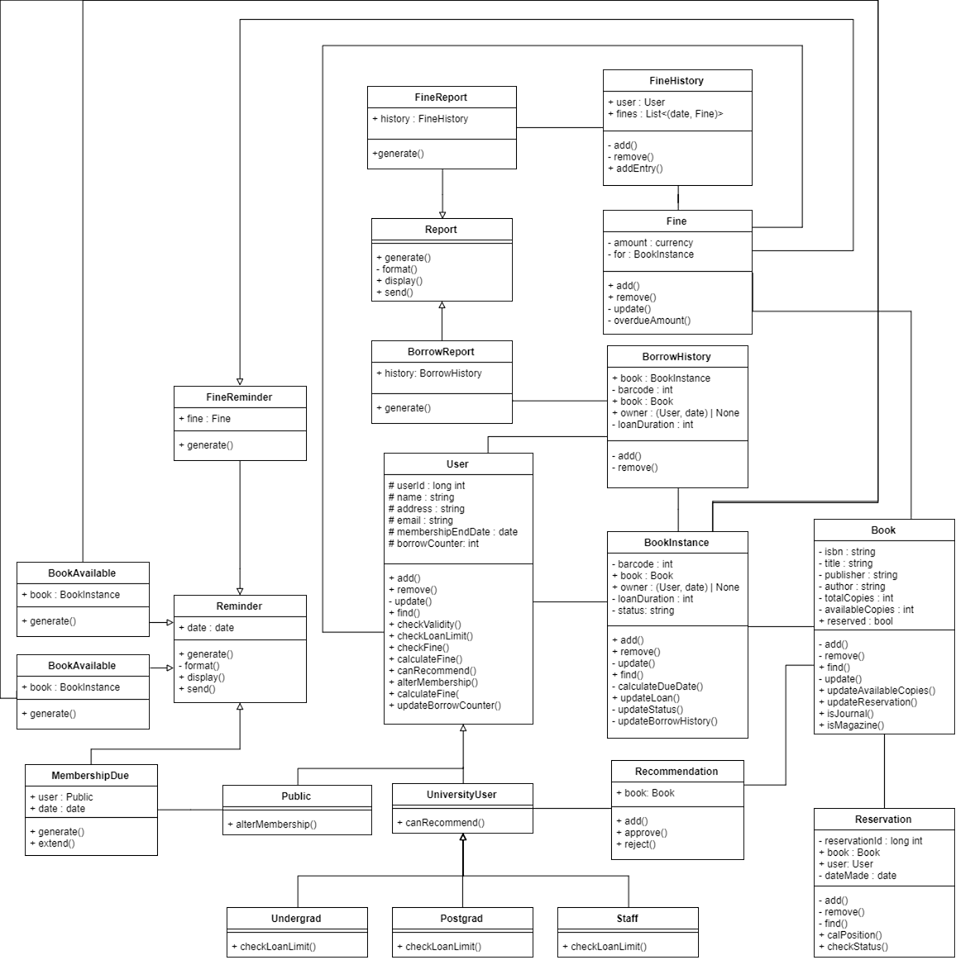
\includegraphics[width=\linewidth]{image/class.png}
    \caption{Class Diagram}
    \label{fig:class}
\end{figure}

\begin{figure}[H]
    \centering
    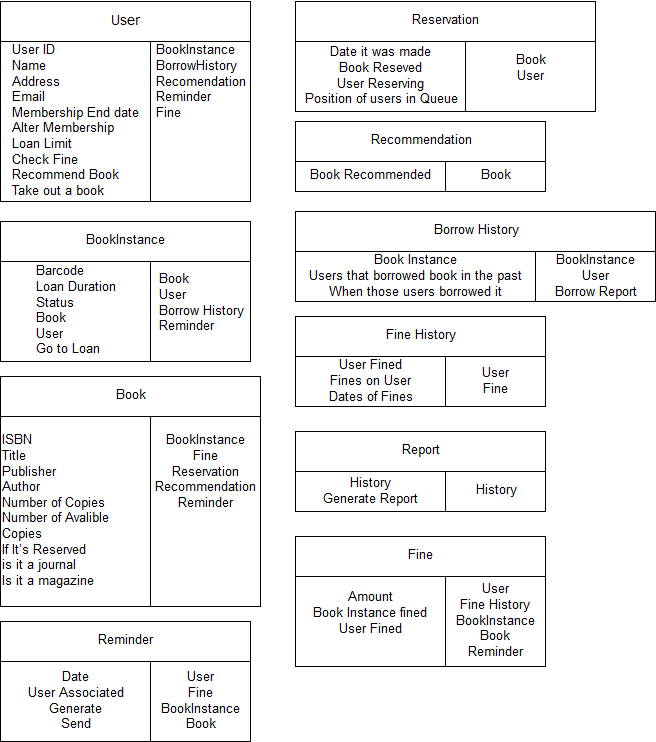
\includegraphics[width=\linewidth]{image/crc.png}
    \caption{Class Responsibility Collaboration Cards}
    \label{fig:crc}
\end{figure}

CRCs are easy to edit and update, and allow designs to stay agile. As they do not link together in a diagram they are more atomic and can be developed without the context of the entire system.

The methods from this diagram are used as connections in sequence model diagrams, and the classes are used as layers. The methods are a more detailed abstraction of what is outlined in the Activity Diagram and Use Case Analysis\cite{ibmclass}. This diagram is useful for understanding the classes used in the system, their attributes, their operations and the types of relationships between different classes. Class diagrams may also be used to further describe the behaviour of systems by extrapolating them to create UML state machines\cite{ambleruml}.